%% Title
\titlepage[of University College London]{%
    A dissertation submitted to University College London\\ for the degree of Doctor of Philosophy}

\begin{figure}
    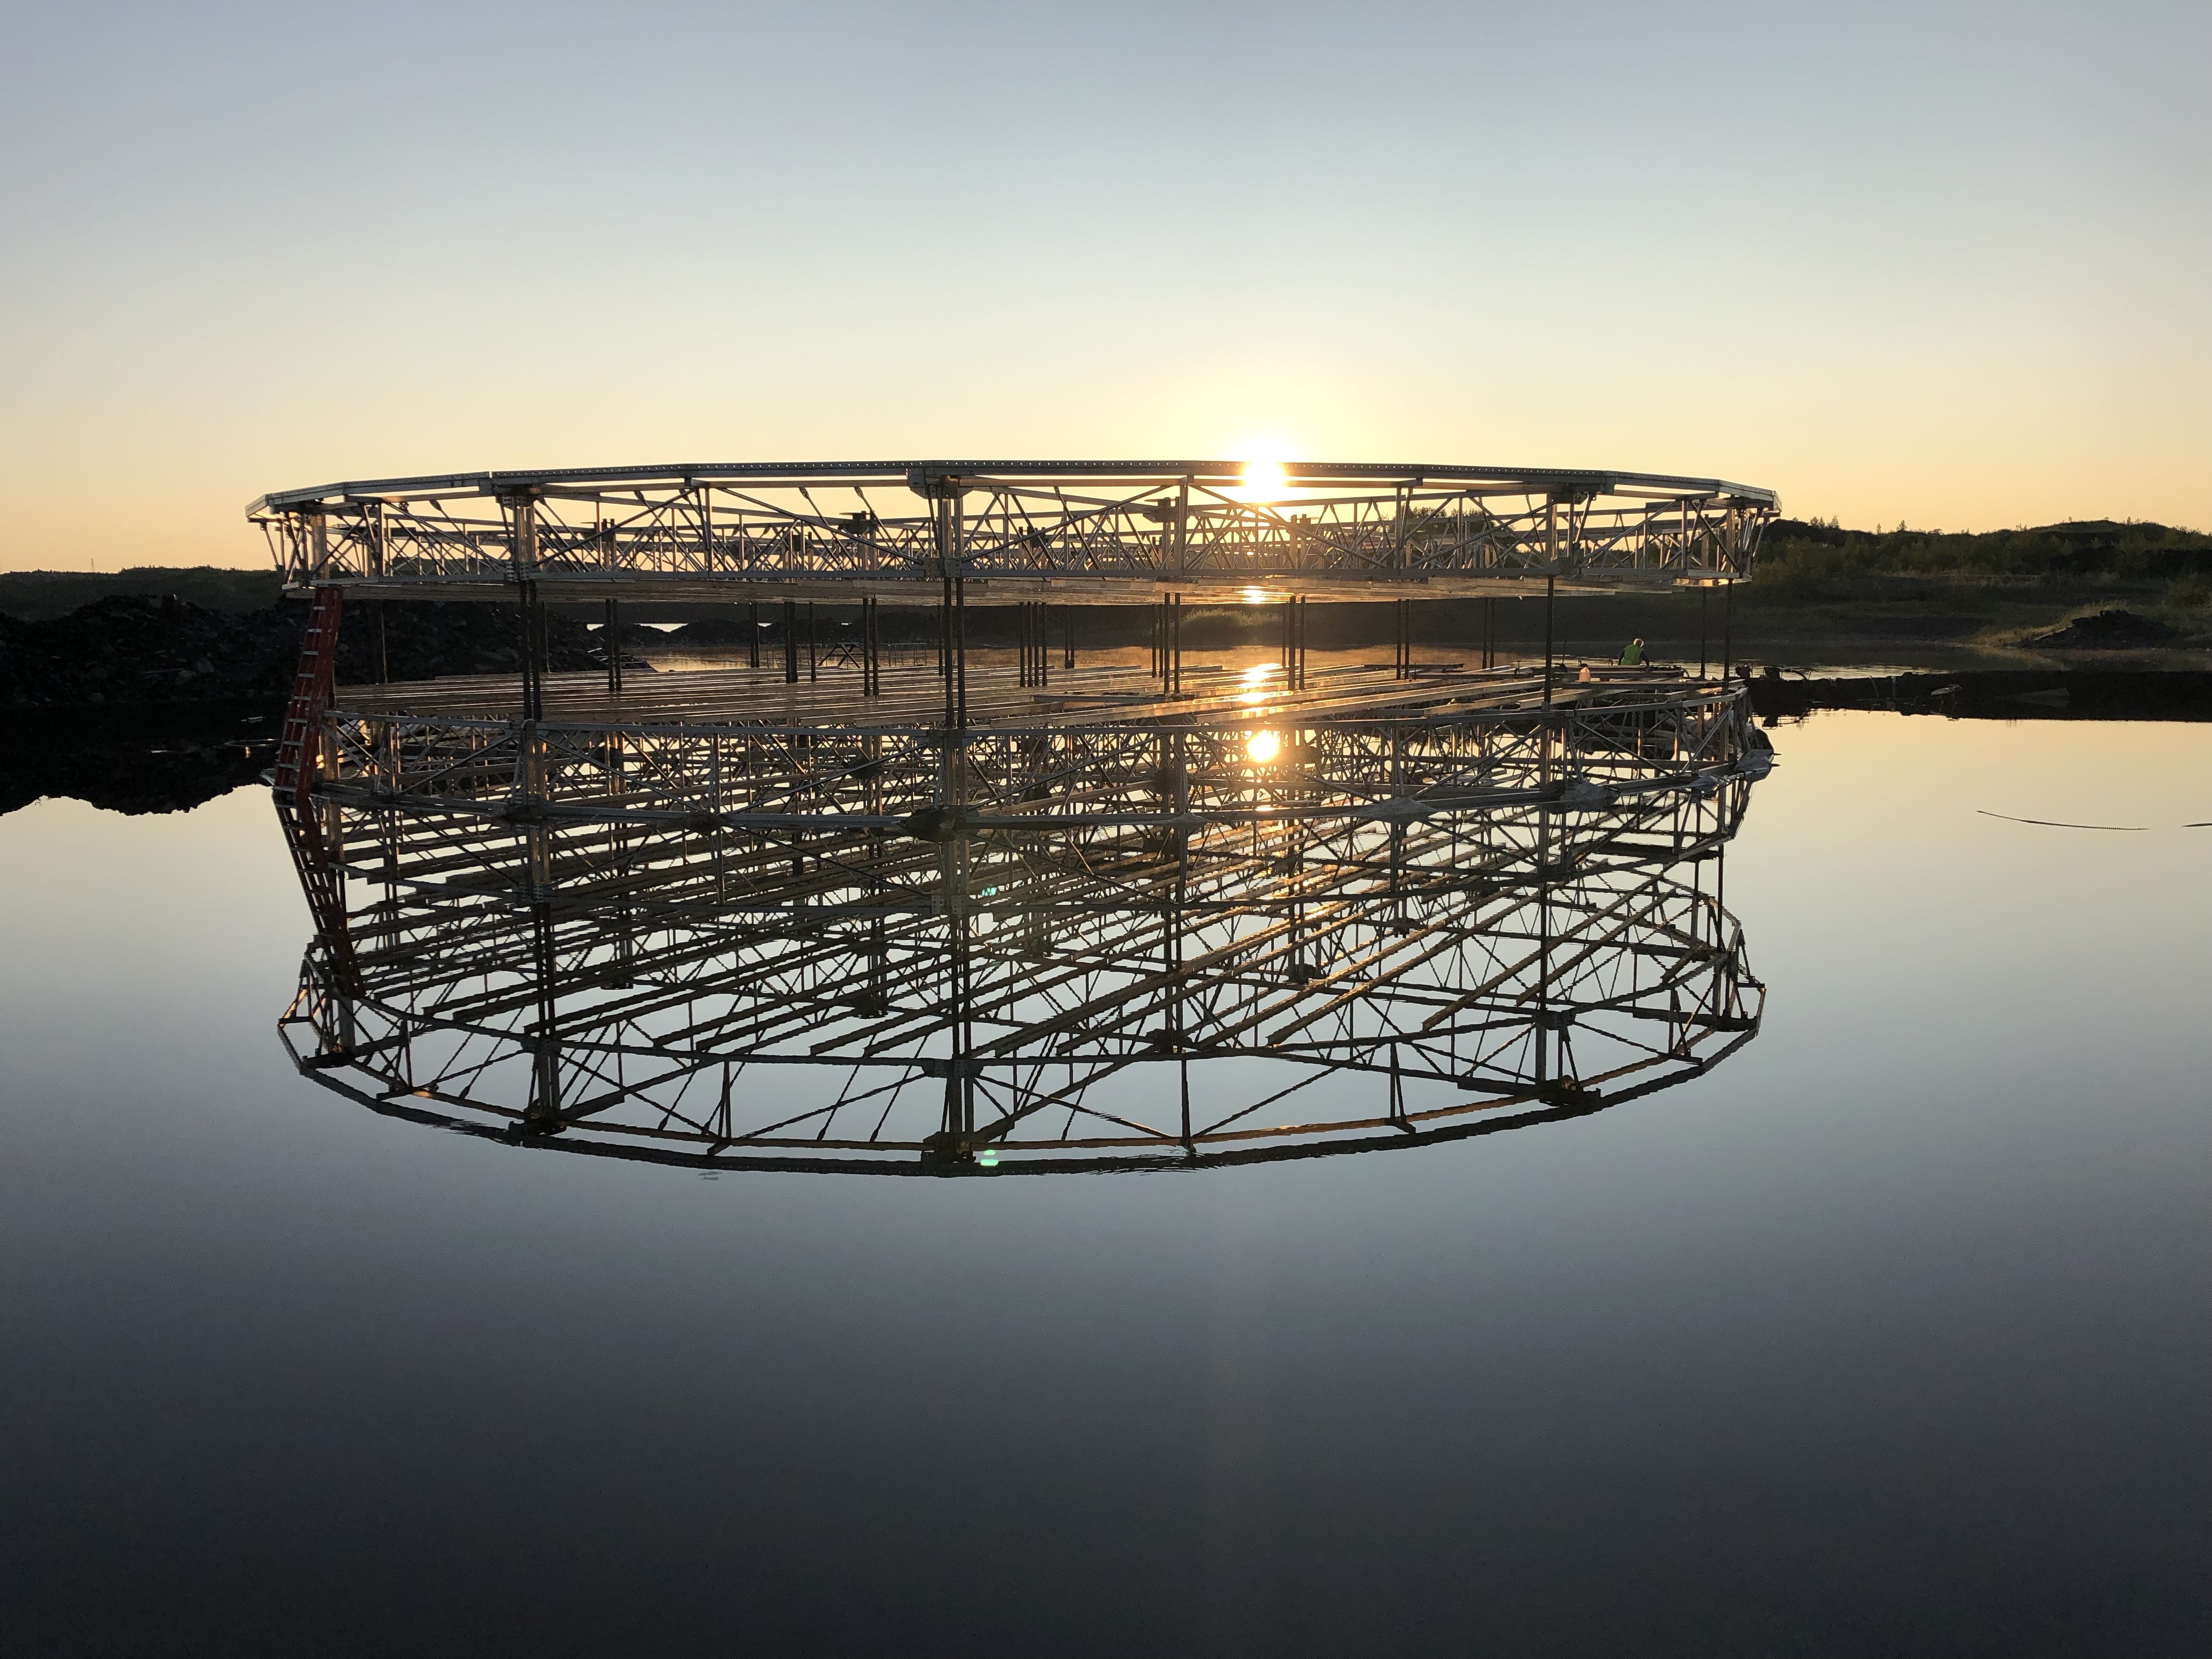
\includegraphics[width=\largefigwidth]{diagrams/sunrise}
\end{figure}

%% Abstract
\begin{abstract}%[\smaller \thetitle\\ \vspace*{1cm} \smaller {\theauthor}]
    %\thispagestyle{empty}
    \LHCb is a \bphysics detector experiment which will take data at
    the \unit{14}{\TeV} \LHC accelerator at \CERN from 2007 onward\dots
\end{abstract}


%% Declaration
\begin{declaration}
    This dissertation is the result of my own work, except where explicit
    reference is made to the work of others, and has not been submitted
    for another qualification to this or any other university. This
    dissertation does not exceed the word limit for the respective Degree
    Committee.
    \vspace*{1cm}
    \begin{flushright}
        Andy Buckley
    \end{flushright}
\end{declaration}


%% Acknowledgements
\begin{acknowledgements}
    Of the many people who deserve thanks, some are particularly prominent,
    such as my supervisor\dots
\end{acknowledgements}


%% Preface
\begin{preface}
    This thesis describes my research on various aspects of the \LHCb
    particle physics program, centred around the \LHCb detector and \LHC
    accelerator at \CERN in Geneva.

    \noindent
    For this example, I'll just mention \ChapterRef{chap:chips}
    and \ChapterRef{chap:theory}.
\end{preface}

%% ToC
\tableofcontents

%% Strictly optional!
\frontquote{%
    Writing in English is the most ingenious torture\\
    ever devised for sins committed in previous lives.}%
{James Joyce}
%% I don't want a page number on the following blank page either.
\thispagestyle{empty}
